\documentclass[11pt]{article}
\usepackage[T1]{fontenc}
\usepackage{lmodern}
\usepackage[a4paper,left=25mm,right=30mm,top=22mm,bottom=24mm,marginparwidth=18mm]{geometry}
\usepackage{amsmath,amssymb,mathtools,stmaryrd}
\usepackage{tikz}
\usetikzlibrary{arrows.meta,calc,positioning}
\usepackage{caption}
\usepackage{xcolor}
\usepackage{marginnote}
\usepackage{microtype}
\usepackage{needspace}
\usepackage[hidelinks]{hyperref}
\definecolor{LeanTeal}{HTML}{087F72}
\definecolor{SourceGray}{HTML}{66736F}
\setlength{\parindent}{0pt}
\setlength{\parskip}{0.55em}
\setlength{\emergencystretch}{2em}
\newcommand{\leanmarker}[2]{%
  \Needspace{3\baselineskip}%
  \marginnote{\hyperlink{#1}{\color{LeanTeal}\fbox{\scriptsize Lean}}}%
  \hypertarget{#1}{\textbf{#2.}}%
}
\newcommand{\sourcepage}[1]{\par\medskip\noindent\textcolor{SourceGray}{\scriptsize Source PDF page #1}\par\smallskip}
\pagestyle{plain}
\begin{document}
\begin{center}\LARGE\bfseries Domains and logic\par\medskip
\large Lean 4 Formalization Companion -- Chapter 7\end{center}
\medskip
\noindent\textit{This project-generated reading copy contains reviewed mathematical items, short source locators, and redrawn diagrams. It does not reproduce the original PDF or automatic OCR prose. Click a Lean tag in the web reader to open the mapped Lean declaration.}
\bigskip\hrule\bigskip
\section*{Section 7.1}
\sourcepage{107}
\leanmarker{thm-7-1-1}{Theorem 7.1.1} A complete lattice \(L\) is continuous if and only if, for every family \((A_i)_{i\in I}\) of directed subsets of \(L\),
\[
  \bigwedge_{i\in I}\bigvee{}^{\uparrow} A_i
  =
  \bigvee_{f:I\overset{\odot}{\longrightarrow}\bigcup_i A_i}^{\uparrow}
    \bigwedge_{i\in I} f(i).
\]

\leanmarker{def-7-1-2}{Definition 7.1.2} For a complete lattice \(L\), define \(x \lll y\) by
\[
  x \lll y \quad\text{iff}\quad
  \forall A\subseteq L,\ \bigl(y\le \bigvee A \Rightarrow \exists a\in A,\ x\le a\bigr).
\]
The lattice \(L\) is prime-continuous if \(x=\bigvee\{y\mid y\lll x\}\) for every \(x\in L\).

\sourcepage{108}
\leanmarker{thm-7-1-3}{Theorem 7.1.3} A complete lattice is prime-continuous if and only if it is completely distributive.

\leanmarker{def-7-1-4}{Definition 7.1.4} A complete lattice \(L\) is \(\wedge\)-generated by a subset \(A\) if, for every \(x\in L\),
\[
  x = \bigwedge(\uparrow x\cap A).
\]
Dually, one speaks of \(\vee\)-generation.

\leanmarker{def-7-1-5}{Definition 7.1.5} An element \(x\) of a lattice \(L\) is \(\wedge\)-irreducible if \(x=\bigwedge M\) for a finite set \(M\subseteq L\) implies \(x=m\) for some \(m\in M\). It is \(\wedge\)-prime if \(x\ge \bigwedge M\) implies \(x\ge m\) for some \(m\in M\), again for finite \(M\). Allowing arbitrary \(M\subseteq L\) gives the completely \(\wedge\)-irreducible and completely \(\wedge\)-prime notions; the dual notions exchange suprema and infima.

\leanmarker{prop-7-1-6}{Proposition 7.1.6} A \(\wedge\)-prime element is also \(\wedge\)-irreducible. The converse holds if the lattice is distributive.

\leanmarker{thm-7-1-7}{Theorem 7.1.7} A continuous lattice is \(\wedge\)-generated by its set of \(\wedge\)-irreducible elements; an algebraic lattice is \(\wedge\)-generated by its completely \(\wedge\)-irreducible elements. The proof separates \(x\nleq y\) by a Scott-open filter and then applies Zorn's lemma to a maximal element above \(y\) outside the filter.

\leanmarker{thm-7-1-8}{Theorem 7.1.8} If \(L\) is a complete lattice which is \(\wedge\)-generated by \(\wedge\)-prime elements, then \(L\) satisfies
\[
  \bigwedge_{m\in M}\bigvee A_m
  =
  \bigvee_{f:M\overset{\odot}{\longrightarrow}\bigcup_m A_m}
    \bigwedge_{m\in M} f(m)
\]
for finite \(M\), and
\[
  \bigvee_{i\in I}\bigwedge M_i
  =
  \bigwedge_{f:I\overset{\odot}{\longrightarrow}\bigcup_i M_i}
    \bigvee_{i\in I} f(i)
\]
when the sets \(M_i\) are finite.

\sourcepage{109}
\leanmarker{def-7-1-9}{Definition 7.1.9} A frame-homomorphism between complete lattices \(K\) and \(L\) is a map preserving arbitrary suprema and finite infima.

\begin{center}
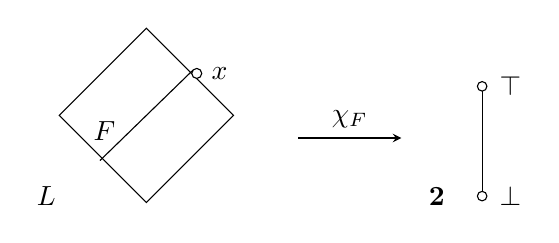
\begin{tikzpicture}[scale=0.82, >=stealth]
  \coordinate (Ltop) at (0,2.25);
  \coordinate (Lright) at (1.35,0.9);
  \coordinate (Lbot) at (0,-0.45);
  \coordinate (Lleft) at (-1.35,0.9);
  \draw (Ltop) -- (Lright) -- (Lbot) -- (Lleft) -- cycle;
  \draw (-0.72,0.2) -- (0.72,1.6);
  \node at (-0.65,0.65) {$F$};
  \node at (-1.55,-0.35) {$L$};
  \filldraw[fill=white] (0.78,1.55) circle (2.2pt);
  \node[right] at (0.86,1.55) {$x$};
  \draw[->] (2.35,0.55) -- node[above] {$\chi_F$} (3.95,0.55);
  \node at (4.5,-0.35) {$\mathbf 2$};
  \draw (5.2,-0.35) -- (5.2,1.35);
  \filldraw[fill=white] (5.2,1.35) circle (2.1pt);
  \filldraw[fill=white] (5.2,-0.35) circle (2.1pt);
  \node[right] at (5.32,1.35) {$\top$};
  \node[right] at (5.32,-0.35) {$\bot$};
\end{tikzpicture}
\end{center}

\sourcepage{110}
\leanmarker{def-7-1-10}{Definition 7.1.10} A filter \(F\subseteq L\) is prime if \(M\in F\) implies \(F\cap M\ne\emptyset\) for every finite \(M\subseteq L\). Allowing arbitrary \(M\) gives completely prime filters. Dually, one has completely prime ideals.

\leanmarker{prop-7-1-11}{Proposition 7.1.11} For a complete lattice \(L\) and subset \(F\subseteq L\), the following are equivalent: \(F\) is a completely prime filter; \(F\) is a filter and \(L\setminus F=\downarrow x\) for some \(x\in L\); \(L\setminus F=\downarrow x\) for a \(\wedge\)-prime element \(x\); and \(\chi_F:L\to \mathbf{2}\) is a frame-homomorphism.

\sourcepage{111}
\leanmarker{def-7-1-12}{Definition 7.1.12} Let \(L\) be a complete lattice. The points of \(L\) are the completely prime filters of \(L\). The collection \(\operatorname{pt}(L)\) is topologized by the basic opens
\[
  O_x = \{F\in\operatorname{pt}(L)\mid x\in F\},\qquad x\in L.
\]

\leanmarker{prop-7-1-13}{Proposition 7.1.13} The sets \(O_x\), \(x\in L\), form a topology on \(\operatorname{pt}(L)\). Indeed, for finite \(M\),
\[
  \bigcap_{m\in M} O_{x_m}=O_{\bigwedge_{m\in M}x_m},
\]
and for arbitrary \(I\),
\[
  \bigcup_{i\in I} O_{x_i}=O_{\bigvee_{i\in I}x_i},
\]
using that points are filters and completely prime filters.

\leanmarker{thm-7-1-14}{Theorem 7.1.14} The functors \(\Omega:\mathbf{Top}\to\mathbf{CLat}\) and \(\operatorname{pt}:\mathbf{CLat}\to\mathbf{Top}\) are dual adjoints. The units are \(\eta\) and \(\epsilon\).

\[
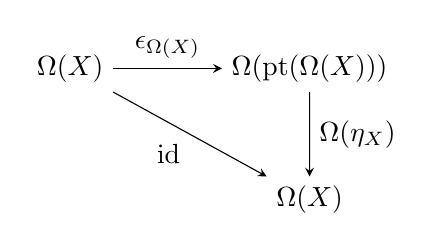
\begin{tikzpicture}[baseline=(current bounding box.center), scale=0.76, >=stealth]
  \node (OX1) at (0,1.4) {$\Omega(X)$};
  \node (OPOX) at (4.0,1.4) {$\Omega(\operatorname{pt}(\Omega(X)))$};
  \node (OX2) at (4.0,-0.8) {$\Omega(X)$};
  \draw[->] (OX1) -- node[above] {$\epsilon_{\Omega(X)}$} (OPOX);
  \draw[->] (OPOX) -- node[right] {$\Omega(\eta_X)$} (OX2);
  \draw[->] (OX1) -- node[below left] {$\operatorname{id}$} (OX2);
\end{tikzpicture}
\qquad\text{and}\qquad
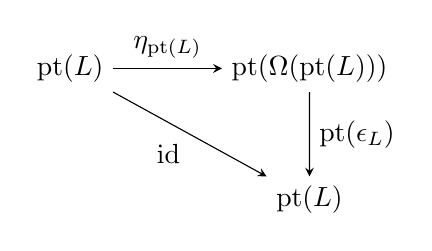
\begin{tikzpicture}[baseline=(current bounding box.center), scale=0.76, >=stealth]
  \node (PL1) at (0,1.4) {$\operatorname{pt}(L)$};
  \node (PPL) at (4.0,1.4) {$\operatorname{pt}(\Omega(\operatorname{pt}(L)))$};
  \node (PL2) at (4.0,-0.8) {$\operatorname{pt}(L)$};
  \draw[->] (PL1) -- node[above] {$\eta_{\operatorname{pt}(L)}$} (PPL);
  \draw[->] (PPL) -- node[right] {$\operatorname{pt}(\epsilon_L)$} (PL2);
  \draw[->] (PL1) -- node[below left] {$\operatorname{id}$} (PL2);
\end{tikzpicture}
\]

\clearpage
\section*{Section 7.2}
\sourcepage{112}
\leanmarker{def-7-2-1}{Definition 7.2.1} A closed subset of a topological space is irreducible if it is non-empty and cannot be written as the union of two closed proper subsets.

\leanmarker{prop-7-2-2}{Proposition 7.2.2} For a topological space \(X\), the unit \(\eta_X:X\to\operatorname{pt}(\Omega(X))\) is injective iff \(X\) is \(T_0\), and it is surjective iff every irreducible closed set is the closure of a point of \(X\).

\sourcepage{113}
\leanmarker{def-7-2-3}{Definition 7.2.3} A topological space \(X\) is sober if \(\eta_X\) is bijective. Equivalently, \(X\) is \(T_0\) and every irreducible closed set is the closure of a unique point.

\leanmarker{prop-7-2-4}{Proposition 7.2.4} For any complete lattice \(L\), the unit \(\epsilon_L:L\to\Omega(\operatorname{pt}(L))\) is surjective and monotone. Moreover, injectivity of \(\epsilon_L\), separation of elements of \(L\) by completely prime filters, and \(\wedge\)-generation of \(L\) by \(\wedge\)-prime elements are equivalent.

\leanmarker{def-7-2-5}{Definition 7.2.5} A complete lattice \(L\) is spatial if \(\epsilon_L\) is bijective.

\leanmarker{thm-7-2-6}{Theorem 7.2.6} A spatial lattice is a frame; in particular it is distributive.

\leanmarker{thm-7-2-7}{Theorem 7.2.7} For every complete lattice \(L\), the space \(\operatorname{pt}(L)\) is sober. For every topological space \(X\), the lattice \(\Omega(X)\) is spatial.

\sourcepage{114}
\leanmarker{cor-7-2-8}{Corollary 7.2.8} The functors \(\Omega\) and \(\operatorname{pt}\) form a dual equivalence between sober spaces and spatial lattices.

\leanmarker{thm-7-2-9}{Theorem 7.2.9} Let \(X\) be sober. The sets of open neighborhoods of compact saturated sets are precisely the Scott-open filters in \(\Omega(X)\).

\sourcepage{115}
\leanmarker{cor-7-2-10}{Corollary 7.2.10} For a sober space \(X\), the poset of compact saturated subsets ordered by inclusion is dually isomorphic to the poset of Scott-open filters in \(\Omega(X)\), also ordered by inclusion.

\leanmarker{cor-7-2-11}{Corollary 7.2.11} In a sober space, filtered intersections of compact saturated subsets are compact; non-empty filtered intersections of non-empty compact saturated subsets are non-empty. If such an intersection is contained in an open set \(O\), then some member of the family is already contained in \(O\).

\leanmarker{prop-7-2-12}{Proposition 7.2.12} For a \(T_0\)-space \(X\), the topology on \(X\) is finer than the weak upper topology induced by the specialization order.

\leanmarker{prop-7-2-13}{Proposition 7.2.13} A sober space is a dcpo in its specialization order, and its topology is coarser than the Scott topology induced by that order.

\leanmarker{thm-7-2-14}{Theorem 7.2.14} The category of sober spaces is complete and cocomplete, and it is closed under retracts formed in the ambient category \(\mathbf{Top}\).

\sourcepage{116}
\leanmarker{lemma-7-2-15}{Lemma 7.2.15} Distributive continuous lattices are spatial.

\leanmarker{thm-7-2-16}{Theorem 7.2.16} The functors \(\Omega\) and \(\operatorname{pt}\) restrict to a dual equivalence between sober locally compact spaces and distributive continuous lattices.

\sourcepage{117}
\leanmarker{def-7-2-17}{Definition 7.2.17} A topological space is coherent if it is sober, locally compact, and the intersection of two compact saturated subsets is compact.

\leanmarker{def-7-2-18}{Definition 7.2.18} The order of approximation on a complete lattice is multiplicative if \(x\ll y\) and \(x\ll z\) imply \(x\ll y\wedge z\). A distributive continuous lattice with multiplicative approximation is arithmetic.

\leanmarker{thm-7-2-19}{Theorem 7.2.19} The functors \(\Omega\) and \(\operatorname{pt}\) restrict to a dual equivalence between coherent spaces and arithmetic lattices.

\leanmarker{thm-7-2-20}{Theorem 7.2.20} The functors \(\Omega\) and \(\operatorname{pt}\) restrict to a dual equivalence between sober spaces whose points have fundamental systems of compact-open neighborhoods and distributive algebraic lattices.

\leanmarker{def-7-2-21}{Definition 7.2.21} A spectral space is a coherent space in which every point has a fundamental system of compact-open neighborhoods.

\leanmarker{thm-7-2-22}{Theorem 7.2.22} The functors \(\Omega\) and \(\operatorname{pt}\) restrict to a dual equivalence between spectral spaces and algebraic arithmetic lattices.

\leanmarker{prop-7-2-23}{Proposition 7.2.23} If \(L\) is an algebraic arithmetic lattice, then completely prime filters of \(L\) correspond bijectively to prime filters of \(K(L)\). The topology on \(\operatorname{pt}(L)\) is generated by the opens \(O_x\) with \(x\in K(L)\).

\sourcepage{118}
\leanmarker{def-7-2-24}{Definition 7.2.24} A relation \(R\) between lattices \(V\) and \(W\) is join-approximable if:
\[
\begin{aligned}
1.\;& \forall x,x'\in V\ \forall y,y'\in W,\ (x'\ge x\ R\ y\ge y' \Rightarrow x'\ R\ y'),\\[2mm]
2.\;& \forall x\in V\ \forall N\subseteq_{\rm fin} W,\ (\forall y\in N,\ x\ R\ y \Rightarrow x\ R\bigvee N),\\[2mm]
3.\;& \forall M\subseteq_{\rm fin} V\ \forall y\in W,\ (\forall x\in M,\ x\ R\ y \Rightarrow (\bigwedge M)\ R\ y),\\[2mm]
4.\;& \forall M\subseteq_{\rm fin} V\ \forall x\in W,\ (\bigvee M)\ R\ x \Rightarrow \exists N\subseteq_{\rm fin} W,\\
& \qquad x=\bigvee N\ \wedge\ \forall n\in N\ \exists m\in M,\ m\ R\ n.
\end{aligned}
\]

\leanmarker{prop-7-2-25}{Proposition 7.2.25} Algebraic arithmetic lattices with frame-homomorphisms are equivalent to distributive lattices with join-approximable relations.

\leanmarker{thm-7-2-26}{Theorem 7.2.26} Spectral spaces and continuous functions are dually equivalent to distributive lattices and join-approximable relations via the contravariant functors \(K\Omega\) and \(\operatorname{spec}\).

\sourcepage{119}
\leanmarker{prop-7-2-27}{Proposition 7.2.27} Continuous domains equipped with the Scott topology are sober spaces.

\textit{Proof.} Let \(A\) be an irreducible closed set in a continuous domain \(D\), and put \(B=\downarrow A\). The set \(B\) is directed: if \(x,y\in B\), then neither \(D\setminus\uparrow x\) nor \(D\setminus\uparrow y\) contains all of \(A\), and irreducibility yields \(a\in A\cap\uparrow x\cap\uparrow y\). Since \(\uparrow x\cap\uparrow y\) is Scott-open, some \(b\ll a\) also lies in it, giving an upper bound for \(x\) and \(y\). Proposition 2.2.10 then shows that \(A\) is the closure of \(\bigvee{}^{\uparrow}B\).

\leanmarker{thm-7-2-28}{Theorem 7.2.28} The functors \(\Omega\) and \(\operatorname{pt}\) restrict to a dual equivalence between \(\mathbf{CONT}\) and the category of completely distributive lattices.

\textit{Proof sketch.} A Scott-open set \(O\) in a continuous domain \(D\) is the union of the sets \(\uparrow x\), \(x\in O\), and each satisfies \(\uparrow x\lll O\) in \(\sigma D\); complete distributivity follows from Theorem 7.1.3. Conversely, if \(L\) is completely distributive, the points of \(L\), ordered by inclusion of filters, form a dcpo. Every completely prime filter \(F\) is enough approximants: whenever \(x\in F\), prime-continuity gives
\[
  x=\bigvee\{y\mid y\lll x\},
\]
so some \(y\in F\) satisfies \(y\lll x\). Interpolation gives a chain \(y\lll\cdots\lll y_n\lll\cdots\lll y_1\lll x\), and \(\bigcup_{n\in\mathbb{N}}\uparrow y_n\) is a completely prime filter containing \(x\) with infimum in \(F\). Thus \(F'\ll F\) iff \(\bigwedge F'\in F\). The Scott topology on the dcpo of points is then exactly the point topology, with basic opens \(O_x=\{F\mid x\in F\}\).

\sourcepage{120}
\leanmarker{thm-7-2-29}{Theorem 7.2.29} The dual equivalence of Theorem 7.2.26 cuts down to a dual equivalence of coherent algebraic domains and lattices in which every element is the join of finitely many \(\vee\)-primes.

\textit{Proof sketch.} A compact-open set in an algebraic domain \(D\) is a finite union of sets of the form \(\uparrow c\) with \(c\in K(D)\), and these are characterized by being \(\vee\)-irreducible and \(\vee\)-prime. Conversely, if every element of a lattice is a finite join of \(\vee\)-primes, then its ideal completion is completely distributive because a principal ideal generated by a \(\vee\)-prime is completely \(\vee\)-prime.

\leanmarker{thm-7-2-30}{Theorem 7.2.30} A lattice \(V\) is isomorphic to the lattice of compact-open subsets of an F-B-domain if and only if:
\begin{enumerate}
\item \(V\) has a least element;
\item each element of \(V\) is the supremum of finitely many \(\vee\)-primes;
\item for every finite set \(M\) of \(\vee\)-primes there is a finite superset \(N\) of \(\vee\)-primes such that
\[
  \forall A\subseteq M\;\exists B\subseteq N.\quad \bigwedge A=\bigvee B.
\]
\end{enumerate}
The additional requirement that there be a largest element which is also \(\vee\)-prime characterizes the lattices of compact-open subsets of bifinite domains.

\sourcepage{121}
\leanmarker{thm-7-2-31}{Theorem 7.2.31} A lattice \(V\) is isomorphic to the lattice of compact-open subsets of an algebraic bc-domain if and only if it has a least element, each element of \(V\) is the supremum of finitely many \(\vee\)-primes, and the set of \(\vee\)-primes plus least element is closed under finite infima.

\begin{center}
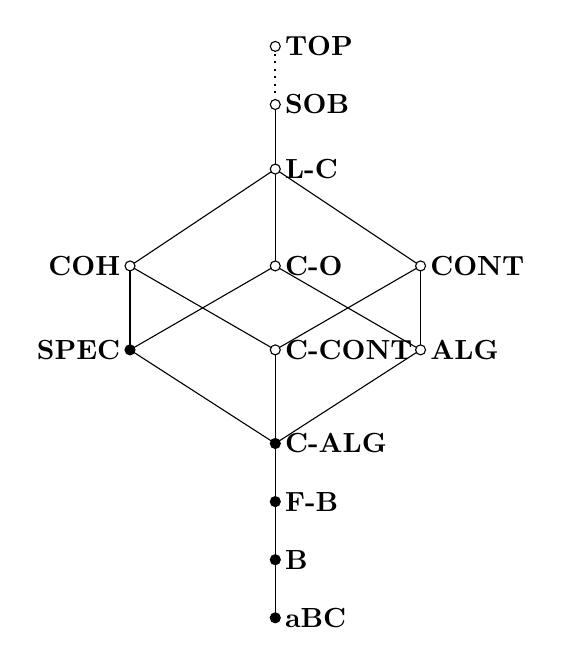
\begin{tikzpicture}[scale=0.82]
  \coordinate (TOP) at (0,5.7);  \coordinate (SOB) at (0,4.8);  \coordinate (LC) at (0,3.8);
  \coordinate (COH) at (-2.25,2.3); \coordinate (CO) at (0,2.3); \coordinate (CONT) at (2.25,2.3);
  \coordinate (SPEC) at (-2.25,1.0); \coordinate (CCONT) at (0,1.0); \coordinate (ALG) at (2.25,1.0);
  \coordinate (CALG) at (0,-0.45); \coordinate (FB) at (0,-1.35); \coordinate (B) at (0,-2.25); \coordinate (aBC) at (0,-3.15);
  \draw[dotted, line width=0.7pt] (TOP) -- (SOB);
  \foreach \u/\v in {SOB/LC,LC/COH,LC/CO,LC/CONT,COH/SPEC,CONT/ALG,COH/CCONT,CONT/CCONT,CO/SPEC,CO/ALG,SPEC/CALG,ALG/CALG,CCONT/CALG,CALG/FB,FB/B,B/aBC} {
    \draw (\u) -- (\v);
  }
  \foreach \p in {TOP,SOB,LC,COH,CO,CONT,CCONT,ALG} {\filldraw[fill=white] (\p) circle (2.2pt);}
  \foreach \p in {SPEC,CALG,FB,B,aBC} {\filldraw[fill=black] (\p) circle (2.2pt);}
  \node[right] at (TOP) {\textbf{TOP}};
  \node[right] at (SOB) {\textbf{SOB}};
  \node[right] at (LC) {\textbf{L-C}};
  \node[left] at (COH) {\textbf{COH}};
  \node[right] at (CO) {\textbf{C-O}};
  \node[right] at (CONT) {\textbf{CONT}};
  \node[left] at (SPEC) {\textbf{SPEC}};
  \node[right] at (CCONT) {\textbf{C-CONT}};
  \node[right] at (ALG) {\textbf{ALG}};
  \node[right] at (CALG) {\textbf{C-ALG}};
  \node[right] at (FB) {\textbf{F-B}};
  \node[right] at (B) {\textbf{B}};
  \node[right] at (aBC) {\textbf{aBC}};
\end{tikzpicture}
\end{center}

\clearpage
\section*{Section 7.3}
\sourcepage{123}
\leanmarker{def-7-3-1}{Definition 7.3.1} A coherent algebraic prelocale \(A\) is a preordered algebra with two binary operations \(\vee\) and \(\wedge\), two nullary operations \(0\) and \(1\), and a unary predicate \(C\) on \(A\), such that \(a\vee b\) is a supremum for \(\{a,b\}\), \(a\wedge b\) is an infimum for \(\{a,b\}\), \(0\) is least, and \(1\) is largest. The preorder is denoted by \(\preceq\), with associated equivalence \(\approx\). The predicate \(C(a)\) holds exactly when \(a\) is \(\vee\)-prime, and every element of \(A\) is equivalent to a finite join of \(\vee\)-primes. Write
\[
  C(A)=\{a\in A\mid C(a)\}.
\]
A \emph{domain prelocale} is a coherent algebraic prelocale satisfying the two additional conditions from Theorem 7.2.30:
\[
\begin{array}{l}
\forall u\subseteq_{\mathrm{fin}}C(A)\ \exists v\subseteq_{\mathrm{fin}}C(A).\ u\subseteq v\ \text{ and }\ (\forall w\subseteq v\ \exists z\subseteq v.\ \bigwedge w=\bigvee z),\\[1mm]
C(1).
\end{array}
\]

\sourcepage{124}
\leanmarker{def-7-3-2}{Definition 7.3.2} Let \(A\) and \(B\) be domain prelocales. A function \(\phi:A\to B\) is a \emph{pre-isomorphism} if it is surjective, order-preserving, and order-reflecting. If \(A\) is a domain prelocale, \(D\) is a bifinite domain, and there is a pre-isomorphism
\[
  \llbracket\cdot\rrbracket:A\to K\Omega(D),
\]
then \(A\) is called a localic description of \(D\) via \(\llbracket\cdot\rrbracket\). A pre-isomorphism preserves suprema, infima, and least and largest elements up to equivalence, and it restricts to a surjective map \(\phi^0:C(A)\to C(B)\).

For \(\llbracket\cdot\rrbracket:A\to K\Omega(D)\), the compact-prime part is compared with compact elements by the dual isomorphism \(K(D)\cong C(K\Omega(D))\):
\[
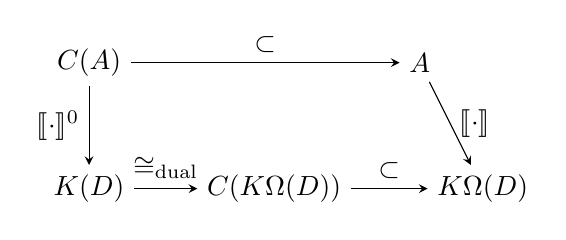
\begin{tikzpicture}[baseline=(current bounding box.center), >=stealth]
  \node (CA) at (0,1.6) {$C(A)$};
  \node (A)  at (4.2,1.6) {$A$};
  \node (KD) at (0,0) {$K(D)$};
  \node (CKO) at (2.35,0) {$C(K\Omega(D))$};
  \node (KO) at (5.0,0) {$K\Omega(D)$};
  \draw[->] (CA) -- node[above] {$\subset$} (A);
  \draw[->] (CA) -- node[left] {$\llbracket\cdot\rrbracket^0$} (KD);
  \draw[->] (A) -- node[right] {$\llbracket\cdot\rrbracket$} (KO);
  \draw[->] (KD) -- node[above] {$\cong_{\mathrm{dual}}$} (CKO);
  \draw[->] (CKO) -- node[above] {$\subset$} (KO);
\end{tikzpicture}
\]

\sourcepage{125}
\leanmarker{prop-7-3-3}{Proposition 7.3.3} There exists a map \(\llbracket\cdot\rrbracket:A\to K\Omega(D)\) such that the domain prelocale \(A\) is a localic description of the bifinite domain \(D\) if and only if \(\operatorname{spec}(A)\) and \(D\) are isomorphic.

\textit{Proof sketch.} A pre-isomorphism yields an isomorphism \(\operatorname{spec}(A)\to D\) by composing \(\operatorname{spec}(\llbracket\cdot\rrbracket)^{-1}\) with the inverse of the unit \(\eta\). Conversely, the unit \(\epsilon:A\to K\Omega(\operatorname{spec}(A))\) is surjective, order-preserving, and order-reflecting by Proposition 7.2.4.

\leanmarker{thm-7-3-4}{Theorem 7.3.4} The category of domain prelocales and join-approximable relations is dually equivalent to the category of bifinite domains and Scott-continuous functions.

\leanmarker{def-7-3-5}{Definition 7.3.5} Let \(A\) and \(B\) be domain prelocales. We say that \(A\) is a sub-prelocale of \(B\) if:
\begin{enumerate}
\item \(A\) is a subalgebra of \(B\) with respect to \(\vee,\wedge,0,1\);
\item the preorder on \(A\) is the restriction of the preorder on \(B\) to \(A\);
\item \(C(A)=A\cap C(B)\).
\end{enumerate}
We write \(A\preccurlyeq B\) if \(A\) is a sub-prelocale of \(B\).

\sourcepage{126}
\leanmarker{prop-7-3-6}{Proposition 7.3.6} If \(A\) is a sub-prelocale of \(B\), then the following maps define an embedding-projection pair between \(\operatorname{spec}(A)\) and \(\operatorname{spec}(B)\):
\[
\begin{array}{ll}
e:\operatorname{spec}(A)\to\operatorname{spec}(B), & e(F)=\uparrow_B(F),\\[1mm]
p:\operatorname{spec}(B)\to\operatorname{spec}(A), & p(F)=F\cap A.
\end{array}
\]
\textit{Proof sketch.} Directed joins of prime filters are directed unions, so both maps are continuous. The identity \(p\circ e=\operatorname{id}\) follows because the preorder on \(A\) is the restriction of that on \(B\), and \(e\circ p\sqsubseteq\operatorname{id}\) needs no special assumptions. The main point is well-definedness: the filter property follows from the inherited operations and preorder, and primeness follows because the \(\vee\)-prime elements of \(A\) are precisely the \(\vee\)-prime elements of \(B\) lying in \(A\).

\leanmarker{cor-7-3-7}{Corollary 7.3.7} Assume that \(A\) is a localic description of \(D\) via \(\llbracket\cdot\rrbracket_A\), that \(B\) describes \(E\) via \(\llbracket\cdot\rrbracket_B\), and that \(A\preccurlyeq B\). Then the following defines an embedding of \(D\) into \(E\): if \(c\in K(D)\), \(a\in C(A)\), \(\llbracket a\rrbracket_A^0=\uparrow c\), and \(\llbracket a\rrbracket_B^0=\uparrow d\), then \(e(c)=d\).

The proof identifies this embedding as \(\tau_B\circ e'\circ\tau_A^{-1}\), where \(e'\) is the embedding \(\operatorname{spec}(A)\to\operatorname{spec}(B)\) from Proposition 7.3.6.

\sourcepage{130}
\leanmarker{lemma-7-3-8}{Lemma 7.3.8} The Scott topology on the function space \([D\to D']\), for bifinite domains \(D\) and \(D'\), equals the compact-open topology.

\textit{Proof sketch.} If \(A\subseteq D\) is compact and \(O\subseteq D'\) is open, then \((A\Rightarrow O)=\{f\mid f(A)\subseteq O\}\) is Scott-open: compactness of \(A\) reduces directed suprema pointwise to finitely many inverse images. Conversely, every Scott-open neighborhood of a function contains a compact-open neighborhood obtained from idempotent deflations on \(D\) and \(D'\).

\leanmarker{lemma-7-3-9}{Lemma 7.3.9} Let \(D\) and \(D'\) be bifinite, and let \(A\subseteq D\) and \(A'\subseteq D'\) be compact-open. Then
\[
  (A\Rightarrow A')=\{f\in[D\to D']\mid f(A)\subseteq A'\}
\]
is compact-open in \([D\to D']\).

\textit{Proof sketch.} By Lemma 7.3.8 this set is open. Bifiniteness supplies idempotent deflations \(g_n\) on \(D\) and \(g'_m\) on \(D'\) with \(A=\uparrow g_n(A)\) and \(A'=\uparrow g'_m(A')\). The induced idempotent deflation \(G_{nm}(f)=g'_m\circ f\circ g_n\) satisfies \((A\Rightarrow A')=\uparrow G_{nm}(A\Rightarrow A')\).

\sourcepage{132}
\leanmarker{thm-7-3-10}{Theorem 7.3.10} Let \(A\) and \(B\) be domain prelocales. Then
\[
  [\operatorname{spec}(A)\to\operatorname{spec}(B)]\cong \operatorname{spec}([A\to B]),
\]
and this isomorphism is natural with respect to the sub-prelocale relation.

\sourcepage{133}
\leanmarker{lemma-7-3-11}{Lemma 7.3.11} If \(D\) is a bifinite domain and \(O\) is compact-open in \(D\), then the following are compact-open subsets of \(P^P(D)\):
\[
\begin{aligned}
  A(O) &= \{L\in\operatorname{Lens}(D)\mid L\subseteq O\},\\
  E(O) &= \{L\in\operatorname{Lens}(D)\mid L\cap O\ne\emptyset\}.
\end{aligned}
\]
Moreover, as \(O\) ranges over all compact-open subsets of \(D\), the sets \(A(O)\) and \(E(O)\) form a base for the Scott topology on \(P^P(D)\).

\textit{Proof sketch.} For compact-open \(O\), choose an idempotent deflation \(d\) with \(O=\uparrow d(O)\). Its lifted deflation \(\hat d=P^P(d)\) makes both \(A(O)\) and \(E(O)\) compact-open. A compact lens \(K=\operatorname{Cx}(u)\), with finite \(u\subseteq K(D)\), has upper set expressible as \(A(\uparrow u)\cap\bigcap_{c\in u}E(\uparrow c)\).

\leanmarker{def-7-3-12}{Definition 7.3.12} Let \(A\) be a domain prelocale which is a localic description of the bifinite domain \(D\). The Plotkin powerlocale \(P^P(A)\) over \(A\) is the term algebra over the generators
\[
  G_P=\{\Box a\mid a\in A\}\cup\{\Diamond a\mid a\in A\},
\]
with interpretation \(\llbracket\cdot\rrbracket:P^P(A)\to K\Omega(P^P(D))\) defined on generators by
\[
  \llbracket\Box a\rrbracket=A(\llbracket a\rrbracket),
  \qquad
  \llbracket\Diamond a\rrbracket=E(\llbracket a\rrbracket),
\]
and extended to \(P^P(A)\) as a lattice homomorphism. The preorder and \(C\)-predicate are given by the rules displayed below.

\sourcepage{135}
\leanmarker{thm-7-3-13}{Theorem 7.3.13} Let \(A\) be a domain prelocale. Then
\[
  P^P(\operatorname{spec}(A))\cong \operatorname{spec}(P^P(A)),
\]
and this isomorphism is natural with respect to the sub-prelocale relation. The Hoare and Smyth powerdomain prelocales are obtained by eliding the generators and rules referring to \(\Box\), respectively \(\Diamond\).

\sourcepage{136}
\leanmarker{thm-7-3-14}{Theorem 7.3.14} If
\[
  A_0\preccurlyeq A_1\preccurlyeq A_2\preccurlyeq\cdots
\]
is a chain of domain prelocales, then
\[
  \operatorname{spec}\Bigl(\bigcup_{n\in\mathbb{N}}A_n\Bigr)
  \cong
  \operatorname{bilim}(\operatorname{spec}(A_n))_{n\in\mathbb{N}}.
\]

\sourcepage{138}
\leanmarker{thm-7-3-15}{Theorem 7.3.15} If \(\rho_L\) and \(\rho_D\) are environments such that, for every \(X\in TV\), the domain prelocale \(\rho_L(X)\) is a localic description of \(\rho_D(X)\), then for every type expression \(\sigma\), \(\mathcal{I}_L(\sigma;\rho_L)\) is a localic description of \(\mathcal{I}_D(\sigma;\rho_D)\). Equivalently,
\[
  \operatorname{spec}(\mathcal{I}_L(\sigma;\rho_L))
  \cong
  \mathcal{I}_D(\sigma;\rho_D).
\]

\sourcepage{139}
\leanmarker{thm-7-3-16}{Theorem 7.3.16} If \(\sigma\) is a closed type expression, then
\[
  \operatorname{spec}(\mathcal{L}(\sigma))\cong \mathcal{I}_D(\sigma).
\]
This is the closed-type instance of Theorem 7.3.15.

\leanmarker{thm-7-3-17}{Theorem 7.3.17} The language of properties is decidable.

\textit{Proof sketch.} For \(\mathcal{L}(\mathbf{1})\) only combinations of \(\mathrm{true}\) and \(\mathrm{false}\) occur. For composite types, every expression in \(\mathcal{L}(\sigma)\) can effectively be transformed into a finite disjunction of \(\vee\)-primes. Soundness and completeness identify these \(\vee\)-primes with the explicit prime expressions produced by the construction rules, and the preorder between them reduces by structural induction on \(\sigma\) to the preorder in \(\mathcal{L}(\mathbf{1})\).

\sourcepage{143}
\leanmarker{thm-7-3-18}{Theorem 7.3.18} The domain logic is sound and complete. In formula form,
\[
  \forall M,\Gamma,\phi.\quad
  \Gamma\vdash M:\phi
  \quad\Longleftrightarrow\quad
  \Gamma\vDash M:\phi.
\]

\end{document}
